\chapter{Imagefilm}
\section{Film, eine Einleitung}
\begin{quote}
    Ein Bild sagt mehr als tausend Worte
\end{quote}
\begin{flushright}
    Fred R. Barnard
\end{flushright}
Mit diesem Zitat lässt sich die Wichtigkeit des Films als Kommunikationsmittel sehr gut beschreiben. So liefert ein Film nicht nur eine große Menge an Informationen durch Darstellung eines Bildes, sondern kann ein Film auch zeitliche Abläufe vermitteln. Oft haben Filme auch noch das weitere Medium des Tons, welches in sich nochmals mehr Informationen trägt. Ein Film kann deswegen als ein sehr \enquote{dichtes} Informationsträger angesehen werden, da in kurzer Zeit sehr viele Informationen gleichzeitig, teils durch verschiedene Kanäle wie Bild und Ton, übertragen werden. So ergibt auch der Einsatz dieses Mediums für die \ac{MOBTS} Konferenz in Mannheim Sinn.\\

Im Folgendem wird deshalb kurz die Geschichte des Films erläutert, um die Vorteile und die interessante Herkunft dieses Mediums darzustellen. Anschließend wird auf verschiedene Techniken des Filmens eingegangen, welche die Grundlagen der Filmproduktion darstellen. Danach wird auf die Umsetzung des Werbefilms für die \ac{MOBTS} Konferenz eingegangen, welcher anschließend bewertet wird. Zuletzt wird noch in einem Fazit ein kurzer Ausblick gegeben.
\section{Geschichte des Films}
Der Mensch suchte schon seit Ewigkeiten danach, seine Erfahrungen und Erlebnisse visuell darzustellen. So finden sich schon in den frühesten Zivilisationen verschiedenste Darstellungen der Umwelt. Noch bevor der Mensch Schrift erfand, malte er auf Höhlenwände Bilder. Mit dem technischen Fortschritt entwickelte sich auch die Darstellungsformen, sodass Bilder auf Leinwände gemalt wurden, bis schließlich die Fotografie erfunden wurde. Bei der Fotografie wird ein lichtempfindlicher Film durch eine Linse mit Licht bestrahlt, was ein Abbild der Umwelt darstellt.\\
Um das Bild bewegt erscheinen zu lassen, erzeugt ein Film eine Illusion, indem mehrere aufeinanderfolgende Bilder schnell hintereinander dargestellt werden. Dies erscheint dann aber einer Bildrate von 24 Bildern pro Sekunde dem menschlichen Auge als flüssige Bewegung.\autocite{Schmidt.2013}\\
Auf der Suche nach dem allerersten \enquote{Film} gibt es drei wesentliche Kandidaten.\autocite{HeadsUp.} Der chronologisch erste Film wurde 1878 erstellt.\autocite{Muybridge.1878} Das Ziel dieses Films war es, herauszufinden, ob ein Pferd im Galopp jemals mit allen vier Hufen gleichzeitig den Boden verlässt. Dafür fotografierte Edward Muybridge ein Pferd in Palo Alto, Kalifornien im Lauf mehrfach mit verschiedenen Kameras, die entlang der Strecke aufgestellt waren. Diese verschiedenen Fotos wurden dann im Nachhinein schnell hintereinander gezeigt, um zu entdecken, dass ein Pferd mit allen vier Hufen gleichzeitig vom Boden abhebt. Hier war es jedoch nicht die Absicht von Muybridge, ein Bewegtbild zu erzeugen, weshalb dies oft nicht als erster Film angesehen wird.\\
Oft wird der Film Roundhay Garden Scene als der erste Film betitelt.\autocite{LePrince.1888} Der von Louis Amie Augustin Le Prince erstellte Film von 1888 geht zwar lediglich zwei Sekunden, stellt jedoch schon eine zusammenhängende Handlung dar und gilt deswegen als Film.\\
Etwas länger dagegen ist der Film \enquote{Arrival of a Train at A la Ciotat}, im original \enquote{L'Arrivée d'un Train A la Ciotat}, welcher 1895 von den Gebrüdern Lumiere erstellt wurde.\autocite{Lumiere.1895} Dieser 50-sekündige Film zeigt einen einfahrenden Zug, eine bekannte Alltagsszene. Zu diesem Film gibt es die unbestätigte Geschichte, welche besagt, dass die Zuschauer dieses Films von der Illusion in einem solchen Sinne getäuscht wurden, sodass sich Panik breit machte und einige Zuschauer aus Angst aus dem Theater flohen. Auch wenn diese Geschichte vielleicht nicht wahr ist, zeigt sie die Überzeugungskraft des Mediums und die Emotionen, die durch visuelle Einflüsse ausgelöst werden können.\\
Dieses Ziel blieb ein wichtiges Ziel in der Filmkunst und Regisseure versuchen bis heute, wirksam Emotionen in Zuschauern auszulösen.\\
\section{Techniken des Filmens}
\subsection{Framing}
Eine der elementarsten Techniken des Filmes ist die des Framings. Das Framing ist ein großer Teil des Filmemachens und beschäftigt sich damit, wie die Kamera eine Szene darstellt. Dabei geht es sowohl um den die Entfernung, Höhe, Brennweite, Fokuseinstellung, Position sowie um den Winkel der Kamera. Auch spielt hierbei oft das Blocking, also die Position der Schauspieler oder Objekte zueinander eine Rolle.\\
Bei der Aufnahmeweite, auch Shotsize genannt, unterscheidet man zunächst zwischen Landschaftsaufnahmen und Aufnahmen von Personen. Landschaftsaufnahmen wird in der Regel der Name Wide Shot oder Long Shot zugeordnet. Dabei wird noch weiter zwischen einem Extreme Wide Shot oder Extreme Long Shot und einem Long Shot unterschieden.

\begin{figure}[h]
    \centering
    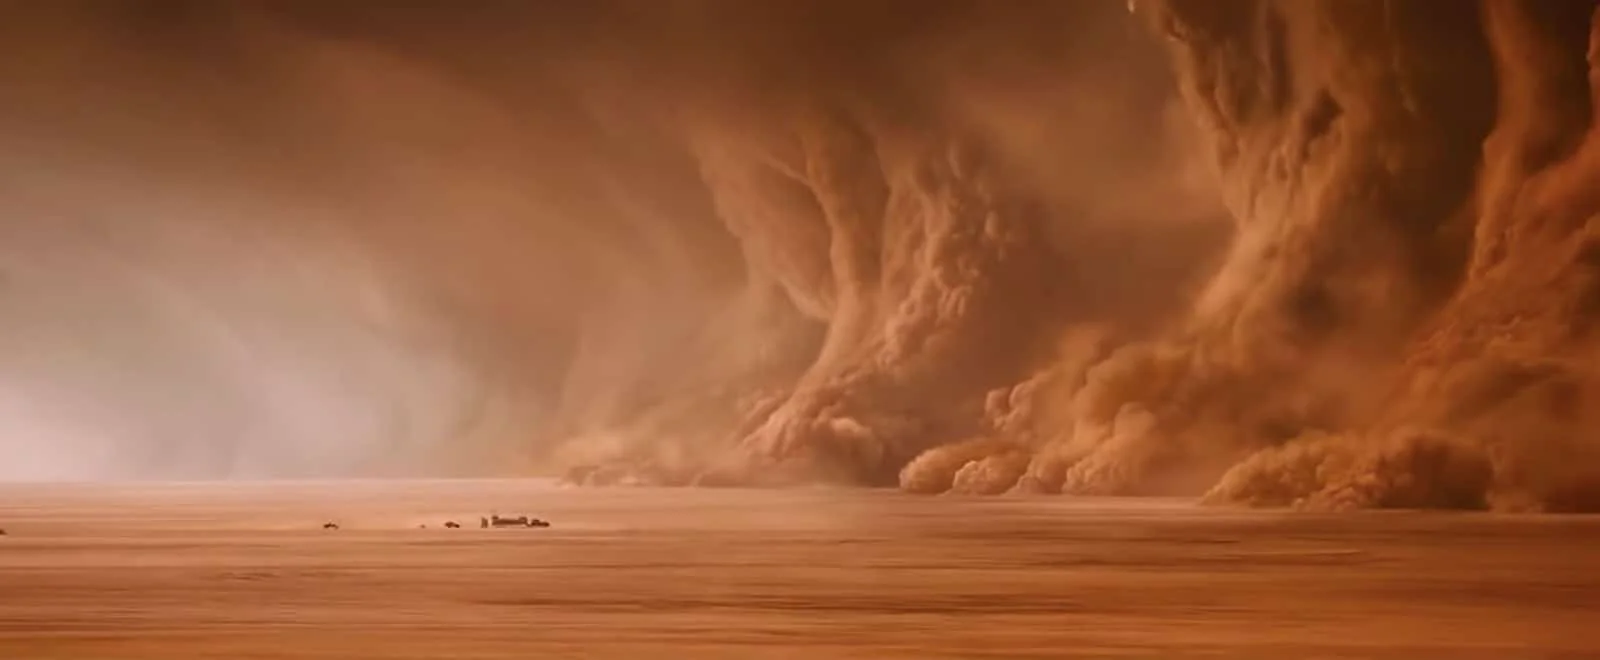
\includegraphics[width=0.8\textwidth]{img/AO_ELS.jpg}
    \caption[Imagefilm: Extreme Wide Shot]{Beispiel eines Extreme Wide Shot (EWS) aus dem Film \textbf{Mad Max: Fury Road}}
    \label{fig:AO_EWS}
\end{figure}

Wie in \autoref{fig:AO_EWS} zu sehen ist, wird in einem Extreme Wide Shot ein großer Teil der Landschaft gezeigt, während kleinere Objekte wie Schauspieler kaum erkennbar sind.\autocite{Studiobinder.2020}

\begin{figure}[h]
    \centering
    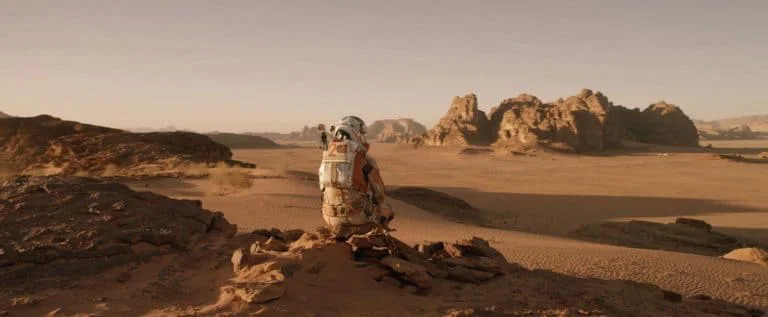
\includegraphics[width=0.8\textwidth]{img/AO_WS.jpg}
    \caption[Imagefilm: Wide Shot]{Beispiel eines Wide Shot (WS) aus dem Film \textbf{Der Marsianer}}
    \label{fig:AO_WS}
\end{figure}

Beim Wide Shot hingegen, wie in \autoref{fig:AO_WS} zu sehen ist, ist der Schauspieler noch gut zu sehen, während der Hintergrund, die Landschaft immer noch betont ist.\\
Diese beiden Aufnahmearten sind die beliebtesten Shots für Landschaftsaufnahmen und können in Verbindung mit anderen Shotarten kombiniert werden, um eine größere Variation von Shots zu erhalten.\\

Bei Personenaufnahmen wird zwischen mehr Shots unterschieden. 

\begin{figure}[h]
    \centering
    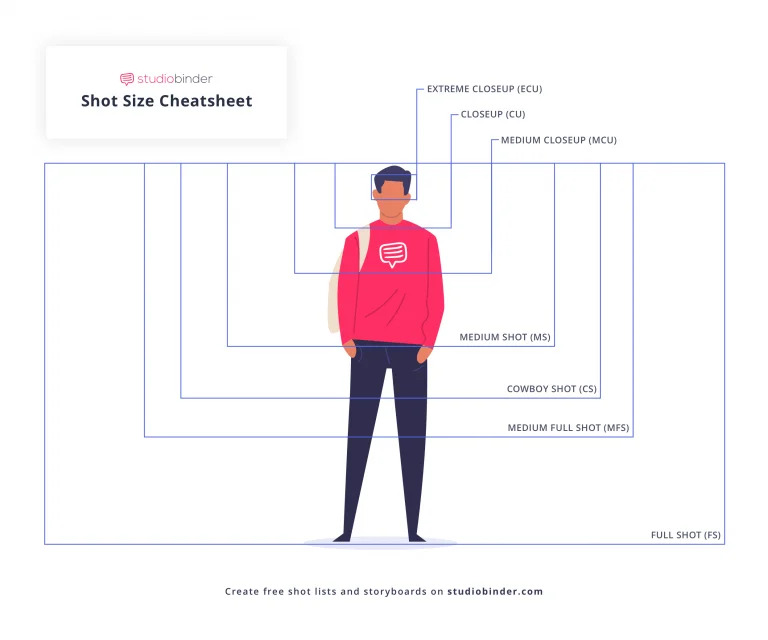
\includegraphics[width=1\textwidth]{img/AO_ShotOverview.jpg}
    \caption[Imagefilm: Shots Übersicht]{Übersicht der bekanntesten Shots für Personen}
    \label{fig:AO_SO}
\end{figure}

Dabei wird in 7 Hauptshots unterschieden, es können aber auch beliebige Zwischenstufen ausgewählt werden, welche dann in der Regel dem naheliegensten Shot zugeordnet wird. 

Der Full Shot ist der weiteste Shot, er zeigt am meisten. In dieser Aufnahme ist der ganze Charakter zu sehen, meistens wird dabei oben und unten noch ein wenig frei gelassen, um es nicht zu eng wirken zu lassen. 

Der nächste Shot ist der Medium Full Shot, hier wird der Charakter von den Knien bis zum Kopf gefilmt. Dieser wird oft benutzt, um Bewegungen eines Charakter zu zeigen.

Beim Cowboy Shot ist der Charakter von etwas unter der Hüfte bis zum Kopf zu sehen. Wie der Name schon sagt, wurde dieser Shot häufig in Western eingesetzt, um sowohl den Charakter als auch den Revolver eines Charakters zu zeigen. Ein Beispiel dafür kann in \autoref{fig:AO_CS} gesehen werden.

\begin{figure}[h]
    \centering
    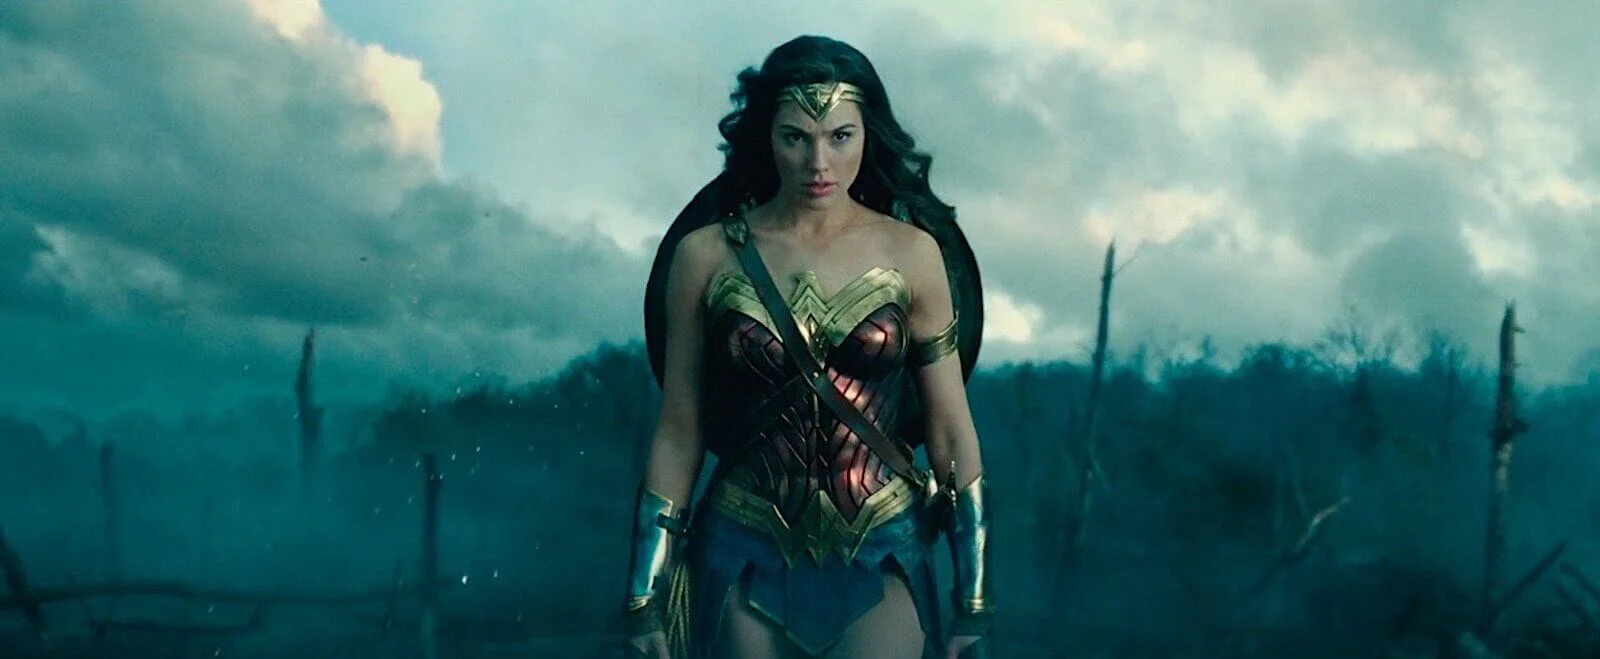
\includegraphics[width=0.8\textwidth]{img/AO_CS.jpg}
    \caption[Imagefilm: Cowboy Shot]{Beispiel für den Cowboy Shot aus dem Film \textbf{Wonder Woman}}
    \label{fig:AO_CS}
\end{figure}

Der Medium Shot wird öfter eingesetzt und zeigt den Charakter von der Hüfte bis zum Kopf. Dieser eignet sich für viele verschiedene Arten von Szenen, da sowohl das Gesicht wie auch der Oberkörper zu sehen ist.

Der Medium Close Up Shot zeigt den Charakter von den Ellenbogen bis zum Kopf und eignet sich somit hervorragend für Konversationen. Das Gesicht und der Oberkörper sind erkennbar, jedoch ist das Bild nicht zu nah, dass es ungemütlich wirkt. Es ist etwa die gleiche Ansicht, die ein Mensch haben würde, wenn er in einer normalen Konversation mit einem anderen Menschen ist. 

Der Close Up dagegen ist wesentlich näher und zeigt meistens nur das Gesicht des Charakters. Er kann auch genutzt werden, um die Detailansicht eines Gegenstandes oder anderen Körperteils zu zeigen. Er wird genutzt, um besondere Aufmerksamkeit auf dieses Objekt zu legen. Bei einem Close Up eines Charakters sollen oft die Emotionen des Charakters betont werden, da bei diesem Shot Gesichtsausdrücke sehr gut erkennbar sind. Das ist in \autoref{fig:AO_CU} zu sehen.

\begin{figure}[h]
    \centering
    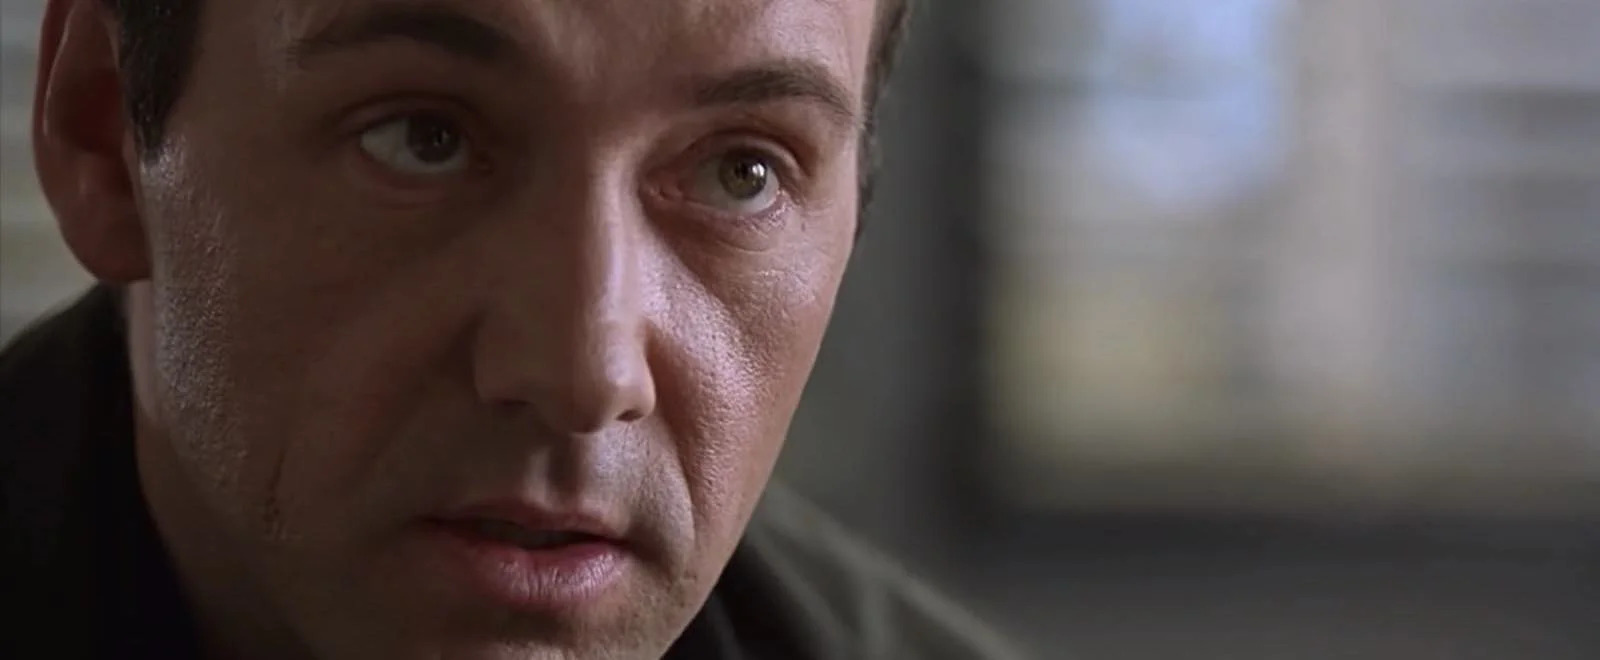
\includegraphics[width=0.8\textwidth]{img/AO_CU.jpg}
    \caption[Imagefilm: Close Up Shot]{Beispiel für den Close-Up Shot aus dem Film \textbf{Die Üblichen Verdächtigen}}
    \label{fig:AO_CU}
\end{figure}

Der Extreme Close Up Shot verstärkt dabei nochmal die Wirkung des Close Up Shots und lenkt somit noch mehr Aufmerksamkeit auf einen bestimmten Aspekt. Oft werden dabei die Augen dargestellt, um eine besonders starke Emotion herauszustellen.

Diese verschiedenen Shotsizes können für unterschiedliche Funktionen innerhalb eines Films genutzt werden.\autocite{Studiobinder.2020}

Eine wichtige Funktion ist dabei der Establishing Shot. Oft wird dieser als eigener Shot dargestellt, es handelt sich jedoch in der Regel um einen Wide Shot oder Extreme Wide Shot. Mit dem Establishing Shot soll eine Szene im Film etabliert werden. Mit diesem Shot soll der Zuschauer orientiert werden und der Schauplatz gezeigt werden. Oft ist es der erste Shot einer Szene oder eines Films.

Weitere wichtige Funktionen sind der Reaction Shot, also eine Aufnahme, die als direkte Reaktion auf die Handlung fungiert, auch Cut-Away genannt, sowie der Over-the-shoulder und Point-of-view shot, welche die Standpunkte der Charaktere besser vermitteln.
\subsection{Goldener Schnitt}
Der Goldene Schnitt ist ein Werkzeug, um ästethisch ansprechende Bilder zu gestalten.\autocite{Bruchwitz.2017}
Der Goldene Schnitt ist dabei eine mathematische Formel. Er beschreibt das Verhältnis von zwei Längen $a$ und $b$ zueinander. Dabei ist $b$ im Verhältnis zu $a$ genau so lang, wie $a$ zu $a + b$ ist. Daraus ergibt sich die Formel
\begin{equation}
    \frac{a}{b} = \frac{a+b}{a}
\end{equation}
Stellt man dieses Verhältnis in die zweite Dimension, so bekommt man ein zwei Rechtecke, welche im Verhältnis des Goldenen Schnittes zueinander stehen. Wenn in dem jeweils kleineren Rechteck auch wieder der Goldenen Schnitt gebildet wird und die Eckpunkte dieser geometrischen Form miteinander verbunden werden, so erhält man die sogenannte Spirale des Nautilus.

\begin{figure}[h]
    \centering
    
\includegraphics[width=0.6\textwidth]{img/AO_GoldenerSchnitt.jpg}
    \caption[Imagefilm: Der Goldene Schnitt]{Die Nautilus Spirale: eine zweidimensionale Darstellung des Goldenen Schnitts}
    \label{fig:AO_GoldenerSchnitt}
\end{figure}

Diese Spirale, wie sie in \autoref{fig:AO_GoldenerSchnitt} zu sehen ist, findet sich, wie auch die Fibonacchi Zahlenfolge, häufig in der Natur.\\
Richtet man Bilder anhand dieses Goldenen Schnittes aus, so werden diese von Menschen als besonders harmonisch empfunden.\autocite{Bruchwitz.2017}\\
Eine vereinfachte Version dieses Goldenen Schnittes wird häufig in der Fotografie sowie in der Videoproduktion genutzt, um Bilder harmonischer wirken zu lassen. Dabei wird das Bild in neun gleichgroße Rechtecke unterteilt, das Bild wird also auf jeder Achse dreigeteilt. Die Schnittstellen dieser Teilungen ergeben dann Markierungen, an welchen Kanten, Objekte und besondere Fokuspunkte ausgerichtet werden können. Diese befinden sich dann annähernd im Goldenen Schnitt und wirken somit harmonisch.\autocite{Bruchwitz.2017}\autocite{HollywoodLexicon.}

\begin{figure}[h]
    \centering
    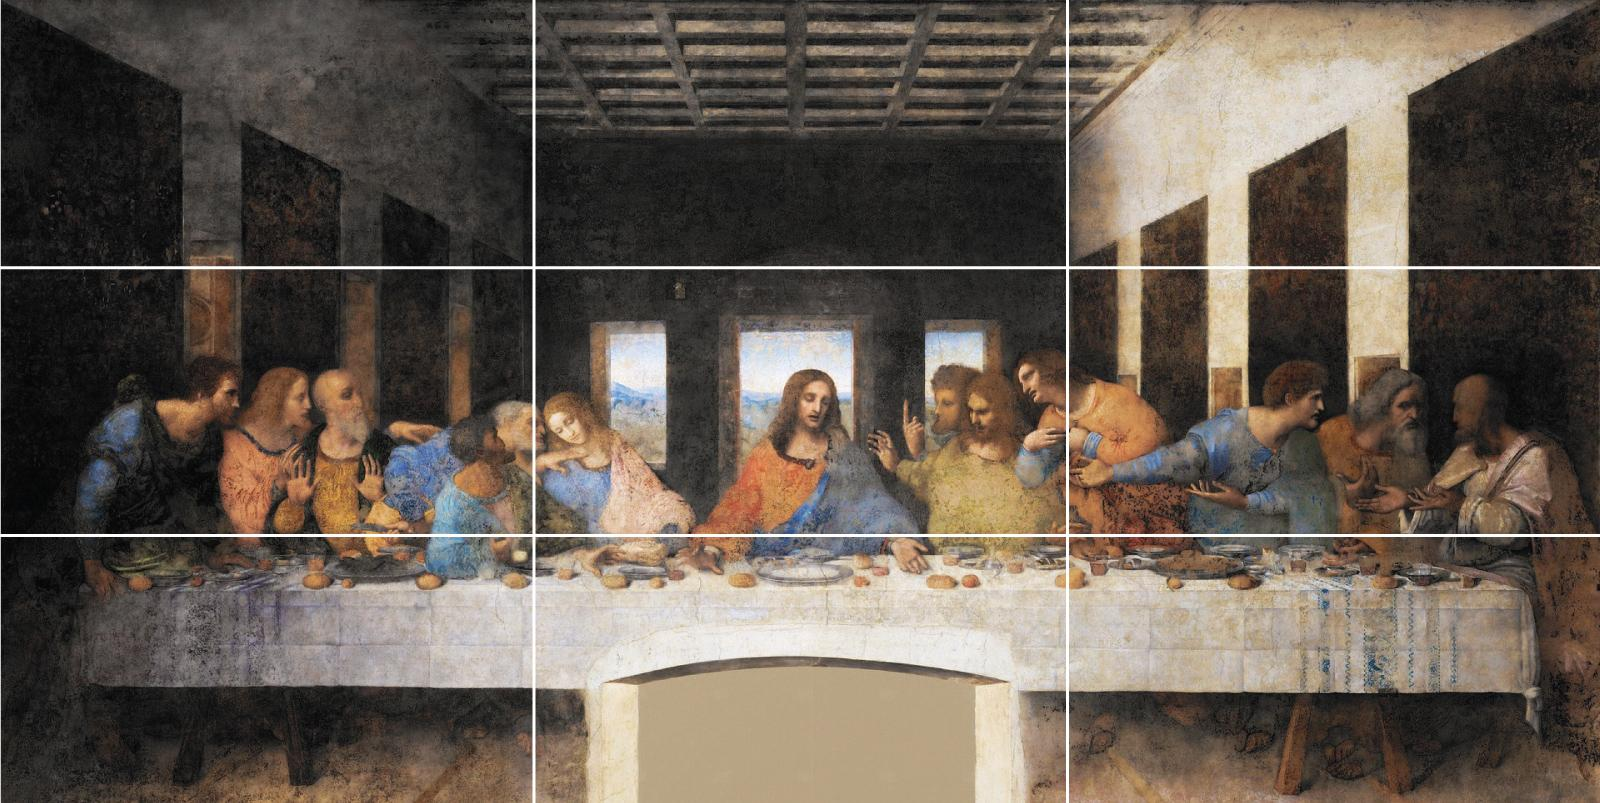
\includegraphics[width=0.8\textwidth]{img/AO_DaVinci.jpg}
    \caption[Imagefilm: Das letzte Abendmahl]{Der Goldene Schnitt wurde schon bei Leonardo DaVincis \textbf{Das letzte Abendmahl} berücksichtigt}
    \label{fig:AO_DaVinci}
\end{figure}

Das ist sogar bei Leonardo DaVincis Bild zu sehen. Wie in \autoref{fig:AO_DaVinci} dargestellt, wird sind die Eckpunkte in diesem Bild zum einen an architekturellen Kanten, auch ist das untere Drittel am Tisch ausgerichtet. Das Bild wirkt dadurch sehr harmonisch und gleichmäßig. 
\subsection{Skript}
Um einen Film koordiniert zu produzieren, ist ein Skript unabdinglich. In einem Skript wird die Handlung des Films festgehalten, sowie alle Dialoge und auch ausgewählte Kamerabewegungen. Dabei unterscheidet sich der Detailgrad des Skripts häufig von Autor zu Autor. So kann auch innerhalb des gleichen Skripts an einer Stelle sehr genau Anweisungen an das Kamera Framing und Blocking sein, während an anderen Stellen gar keine Anweisungen über die aktuelle Kameraposition zu finden ist. Das liegt dann an dem Autor, welche für bestimmte Szenen sehr spezifische Vorstellungen haben kann, für andere jedoch nicht und diese Aufgabe dann indirekt an den Kameramann übergibt. Auch ist dies abhängig vom technischen Know-How des Autors.\\
Das Skript gilt als Leitfaden für den Film und die Länge des Skripts beeinflusst direkt die Länge des Films. Im Skript sollten alles, was im Film vorkommt, beschrieben sein und der Film sollte nur das beinhalten, was im Skript festgelegt wurde, auch wenn kleine Abweichungen vom Skript möglich sind. 
\subsection{Voiceover}
Beim sogenannten Voiceover wird über Bilder und Videos ein Text eingesprochen. Im Regelfall ist dabei das Voice eine inhaltliche Ergänzung zum Bild; oft ist der Ton dabei die Hauptinformationsträger, während das Bild nur als Unterstützung gilt und besonders auf den visuellen Kontext eingeht. \autocite{Schmidt.2013} Auch wird das Bild dabei genutzt, um das Video dem Zuschauer interessanter darzustellen und die geringe Aufmerksamkeitspanne eines Zuschauers zu halten.\\
Oft wird ein Voiceover bei Videos genutzt, welche hauptsächlich zur Informationsübermittlung genutzt werden, sogenannte Infovideos. Hier liest die Stimme des Voiceovers Informationen vor, während Bilder diese Informationen ergänzen, ein Gefühl für das Gesagte vermitteln oder Daten wie Zahlen und Termine visuell darstellen.\\
Beim Bild ist bei einem Voice darauf zu achten, dass es klar ersichtlich ist, was die Bilder und Videos darstellen. Da der Zuschauer gleichzeitig mit dem zuhören und extrahieren von Daten auf der akustischen Spur beschäftigt ist, sollte die visuelle Spur keinen großen Verarbeitungsaufwand darstellen. Außerdem sollte komplizierte Daten, wie Zahlen und Termine, visuell redundant dargestellt werden. Trotz der Einfachheit sollten die Bilder gewünschte Emotionen im Zuschauer auslösen. Bei Infovideos sind diese Emotionen im Regelfall positiv, oft motivierend.\\
Beim Ton ist darauf zu achten, dass der Sprecher deutlich spricht, um hier die Informationsaufnahme einfacher zu gestalten. Jedoch sollte die Stimme nicht zu monoton wirken, es sollte eine Variation in der Modulierung der Stimme sowohl bei Lautstärke wie auch bei Geschwindigkeit auftreten, um Spannung beizubehalten. Zur Deutlichkeit muss der Sprecher langsam reden, jedoch nicht zu langsam, um das Interesse der Zuschauer zu wecken. Erzeugung von Sympathie über die Stimme ist auch ein wichtiger Faktor, um die Zuschauer emotional zu beeinflussen. Diese Faktoren können auch über eine elektronische Veränderung der Stimme erreicht werden. 
\section{Imagefilm zur MOBTS}
\subsection{Ziel des Films}
Im Rahmen der \ac{MOBTS} Eventorganisation soll ein Imagefilm entstehen, welcher sowohl die \ac{MOBTS} 2022 bewirbt, als auch die Stadt Mannheim und die generelle Umgebung dieser Veranstaltung vorstellt. Dabei soll der Zuschauer viele Informationen zur Konferenz bekommen und gleichzeitig Lust und Motivation bekommen, die Konferenz zu besuchen und Mannheim und die Umgebung zu erkunden und sich kulturell beeinflussen zu lassen. Aus diesem Grund wurde die Form des Infovideos für diesen Imagefilm gewählt. Da die \ac{MOBTS} eine internationale Konferenz ist, soll der Imagefilm auf Englisch erstellt werden. Da Englisch die Weltsprache ist, kann dieser Film auch für andere Länder genutzt werden. Eine deutsche Version ist nicht geplant. Der Imagefilm soll dabei grob aus zwei Teilen bestehen, der erste beschreibt die Konferenz, die Themen der Konferenz und den groben Ablauf der Konferenz, während der zweite Teil Mannheim und die Umgebung präsentiert. Am Ende soll dann noch auf die Konferenz zurückgekommen werden, um einen runden Abschluss zu geben. In dem Film soll auch die \ac{MOBTS} als Unternehmen vorgestellt werden. Für den Film wurde ein Skript erstellt, welches größtenteils nur den gesprochenen Text umfasst, da für die Bilder noch kein konkreter Plan vorhanden war.
\subsection{Skript des Films}
Anmerkung: Text in \textit{kursiv} beschreibt Bildanweisung, Text in Normal beschreibt gesprochene Sprache.

\textit{Anfangslogo, kurze Übersicht der Daten}
In June 2022 the MOBTS Conference will take place at the Baden-Wuerttemberg Cooperative State Universities, the DHBW in Mannheim.\\
\textit{Logo der MOBTS}\\
The international MOBTS is a leader in pedagogical management on a global level, as well as being one of the best values you will find at a conference of any kind.\\
\textit{Logo der MOBTS}\\
Their mission is to enhance the quality of teaching and learning across the management disciplines.\\
\textit{Diverse Bilder, die dem Thema entsprechen}\\
In 2022 the conference will be focusing on a very important topic in today’s modern and digital world: Digital learning.\\
\textit{Bilder zum Thema Digital Learning, Menschen die am PC arbeiten}\\
Not only in times of a pandemic is this a very important topic but also in everyday life.\\ 
\textit{Bilder passend zur Pandemie}\\
How can the digital learning experience be successful? How can the digitization in the learning and work environment be driven forward and be improved?\\
\textit{Bilder passend zum Thema, Personen die bei einem Vortrag zuhören}\\
The DHBW had to face the problems of digital learning for itself with the corona pandemic and was able to change to a digital learning environment quickly and successfully.\\
\textit{Bilder passend zum Thema, Menschen die Lernen}\\
That’s why it is the perfect host for the 2022 MOBTS.\\
Don’t miss out on exciting presentations, discussions and workshops about gamification, digital schools and remote working and become an expert in the field of digital learning and remote working.\\
\textit{Bilder, die zum Thema passen und Digital Learning zeigen}\\
Apart from the conference you will be able to take part in great events to get to know Mannheim, the location of the DHBW.\\
\textit{Zoom in von Google Maps auf die Stadt Mannheim}\\
In the city of Mannheim you can expect to encounter anything - except boredom.\\
With a population of approxiately 310.000 inhabitants Mannheim is the second largest town in the German state of Baden-Württemberg.\\
\textit{Übersicht von Mannheim zeigen, Zahl 310.000 einblenden}\\
The special thing about Mannheim is that its avenues and streets are, unlike every other german town, laid out in a grid pattern.\\
\textit{So reinzoomen, dass die Quadrate der Stadt Mannheim ersichtlich sind}\\
That’s why it’s also called “die Quadratestadt” (the Square City).\\
Mannheim also lives innovation. Many ground-breaking inventions have come out of Mannheim.\\
\textit{Bilder von verschiedenen Technologien zeigen}\\ 
In 1886 Carl Benz invented the very first automobile in the world. Two years later his wife drove it from Mannheim to Pforzheim and back.\\
\textit{Bilder von Carl Benz und dem ersten Auto}\\
Moreover in Mannheim the bicycle and the tractor were invented.\\
\textit{Bild von Traktor}\\
A yummy invention was the spaghettieis. It’s a german ice cream dish that consists of vanilla ice cream which looks like spaghetti topped with a strawberry sauce to simulate a tomato sauce.\\
\textit{Bilder von Spaghettieis}\\
The ice cream shop which invented spaghettieis can still be found in downtown Mannheim. You should try it while visiting us.\\
\textit{Zoom von Google Maps auf Standort des Eisladens in Mannheim}\\
Mannheim also has many beautiful buildings and sights.\\
\textit{Zoom over zum Wasserturm}\\
One of them is the water tower which is the symbol of Mannheim. 
Here you can see why Mannheim once was called “Little Paris”.\\
\textit{Bild von Wasserturm}\\
Moreover Mannheim has a baroque castle which accommodates the university of Mannheim nowadays.\\
\textit{Zoom von Wasserturm zur Uni Mannheim}\\
The beautiful neighboring city Heidelberg is also worth seeing while visiting Mannheim with its beautiful castle and old town.\\
\textit{Bilder von Heidelberg}\\ 
Located just 7 km next to the city center of Mannheim is one of the twelve Baden-Wuerttemberg Cooperative State Universities, the DHBW, where the MOBTS conference will take place.\\
\textit{Zoom over von Uni Mannheim zur DHBW Mannheim}\\
It offers higher education in cooperation with industry and non-profit institutions.\\
\textit{Imagebilder von DHBW}\\
This combines on-the-job-training and academic studies.\\
With around 34.000 enrolled students, over 9.000 partner companies and more than 145.000 graduates, the university counts as one of the largest higher education institutions in the german state of Baden-Württemberg.\\
\textit{Weitere Imagebilder der DHBW, einblendung der Zahlen}\\
Both the airport of Frankfurt and Stuttgart are not far and can be easily reached by Train and car which makes the DHBW a perfect location for the conference.\\
\textit{Darstellung der Fahrtzeiten von Frankfurt und Stuttgart zur DHBW}\\
Don’t miss out on exciting presentations and workshops and visit the beautiful city of Mannheim.\\
\textit{Weitere Imagevideos}\\
Become an expert in the field of digital learning and remote working and stay up to date in the modern world.\\ 
The conference will take place from the 23rd of June to the 25th of June.\\
\textit{Einblenden der Termine}\\
Save the date and get your tickets now.\\
More information can be found on the MOBTS Website\\
\textit{Einblendung der Website, Endbild, Schluss}
\subsection{Durchführung und Produktion}
Für die Produktion wurde zuerst die Tonspur erzeugt, um dann die Bilder passend dazu zu gestalten. Dazu wurden die einzelnen Zeilen des Skripts separat aufgenommen, um eine Bearbeitung im Nachhinein einfacher zu gestalten.\\
Das Voiceover wurde dabei mit einem Großmembran-Kondensatormikrofon aufgenommen, um sowohl gute Audioqualität zu erlangen, wie auch eine besondere Wärme der Stimme durch das basslastige Aufnahmemuster zu erzeugen. Zusätzlich wurden noch drei weitere Effekte auf die Tonspur gelegt. Zuerst wurde für die jeweilige Aufnahme eine Rauschentfernung durchgeführt. Dies wird gemacht, um die restlichen Hintergrundgeräusche die verbleiben, auszublenden. Als Nächstes wird ein Equalizer auf die Audiospur angewendet. Mit diesem Equalizer werden die warmen Frequenzen der Stimme verstärkt, während andere, störende Frequenzen, wie stark betonte S und P laute ausgefiltert werden. Als Letztes wird noch ein Kompressor mit anschließender Normalisierung angewendet. Ein Kompressor stellt ab einem bestimmten Limit leise Töne lauter und laute Töne leiser. Dadurch wirkt der Text verständlicher und er kann leichter wahrgenommen werden. Auch hat dies den Effekt, dass sich der gesprochene Text über die Hintergrundmusik abhebt und auch bei geringeren Lautstärken einfacher verständlich ist.\\
Für die Videospur wurde zunächst eine Tour in Google Earth erstellt, um die Vogelperspektiven und Außenansichten von Mannheim zu zeigen. Dann wurden diverse Bilder aus der Bilddatenbank Mannheim, aus der Uni Imagebibliothek sowie aus kostenlos verfügbaren lizenzfreien Stock-footage Bibliotheken genommen und diese passend zum jeweiligen gesprochenen Text geschnitten. Das Schneiden fand über HitFilm 3 Express statt und das Video wurde im mp4 Format gerendert. Somit kann es auf den meisten Videoplattformen eingebettet werden.
\section{Fazit und Ausblick}
Zusammenfassend ist der Film ein starkes Mittel, um Emotionen bei Zuschauern auszulösen. Das Infovideo ist ein gutes Mittel, um schnell Informationen einfach und angenehm zu übertragen und eignet sich gut als Marketingtool. Auch ist die vielseitige Einsetzbarkeit zu beachten.\\
Des Weiteren könnte der Imagefilm der \ac{MOBTS} in verschiedenen Sprachen aufgenommen werden. Auch könnten noch weitere Videos, wie Beispielsweise ein Trailer für die Konferenz, erzeugt werden.
